\section{Udviklingsmetoder}

\subsection{Agil udvikling}
Agil betyder forandringsparathed.
Centrale værdier for agil softwareudvikling.

Individer og interaktioner er vigigere end processer og værktøjer. Software, der virker, er vigtigere end omfattende dokumentation.
Samarbejde med kunden er vigtigere end kontraktforhandling. At kunne reagere på forandringer er vigtigere end at følge en plan.


\textbf{The agile enterprise}
\begin{itemize}
	\item{Der skal være en stærk virksomhedsideologi}
	\item{Der skal være en stærk virksomhedskultur med afsæt i ideologien.}
	\item{Man skal kunne agere proaktivt.}
	\item{Man skal kunne reagere reaktivt.The agile enterprise}
	\item{Forandringsparathed skal kunne måles}
	\item{Virksomheden skal råde over en række genbrugelige komponenter, som nemt kan kombineres.}
	\item{Ovennævnte plug-in kompatibilitet understøttes aktivt af udviklende standarder.}
	\item{Medarbejderne skal kunne eksperimentere frit i selvorganiserende grupper}
	\item{Virksomheden skal facilitere videndeling.}
	\item {Koordinering finder sted på individniveau}
\end{itemize}

\subsection{Kanban}
Kanban er en metode til at styre flowet af arbejdet. Man bruger "noter" på "tavler" til at visualisere og holde styr på projektet.

\begin{center}
	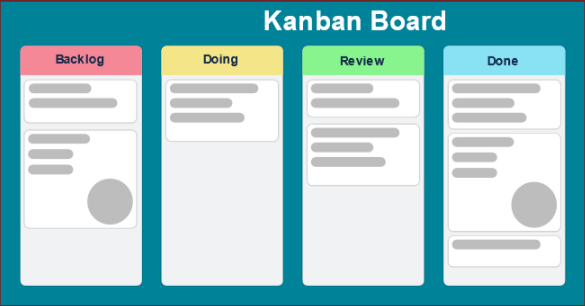
\includegraphics[width=0.8\textwidth]{Images/Kanban.png}
\end{center}

Ved Kanban har man et commitment point, hvor vi beslutter os for at det skal udføres.
Dertil er der lead time, som er hvor lang tid det tager at gennemføre. En vigtig begrænsing er  WIP limits.
Work in progress limits sikrer at man færdiggører opgaver og ikke bare tilføjer flere.


\subsection{Rubber duck debugging}
Ved at forklare sit problem kan man bedre forstå det.

\subsection{Extreme programming}
Vi prøver ikke at at forudse alt hvad der skal laves. I stedet fokuseres
der på det mest værdifulde og så starter vi der. Da der ikke er lavet
overordnede planer er der stor risiko for kaos. Der er derfor oprettet
forskellige regler for at holde styr på kaosset. Det gøres ved forskellige
niveauer af feedback.

\textbf{Pair programming}

I extreme programming programmerer man ikke alene. Man gør det altid i par.
Den ene skriver kode og arbejder med at finde den umiddelbare løsning.
Den anden er "navigatør/observatør" og laver review af koden og er
opmærksom på den længeresigtede planlægning.

\textbf{Stand-up meetings}

Man mødes alle på holdet først om dagen. Mødet foregår stående så det
ikke tager for lang tid. Man fortæller hvad man er i gang med at arbejde på
og om der er problemer. Derved ved hele holdet hvor alle er og muligheder
for samarbejde forbedres.

\textbf{Acceptance tests}
Er det vi har lavet acceptabelt for kunden? Der laves tests for kunden
der viser det nuværende system. Eventuelle uoverensstemmelser kan rettes
hurtigt i projektet.


\begin{center}
	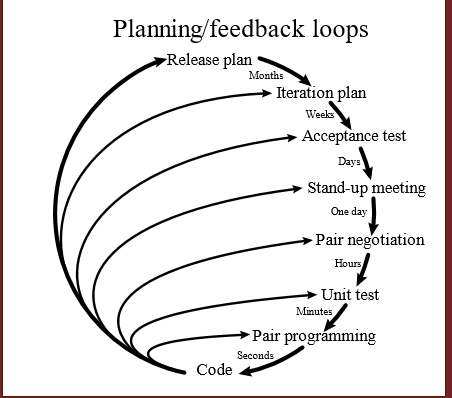
\includegraphics[width=0.5\textwidth]{Images/extreme.png}
\end{center}


\subsection{Vandfaldsmodellen}
Man fortsætter først når forrige skridt er gennemført.
Passer godt med uvikling af systemer, hvor forandringer er dyre. f.eks. udvikling af tog.
Modsat er det næsten umuligt at udvikle et system top-down.


\begin{center}
	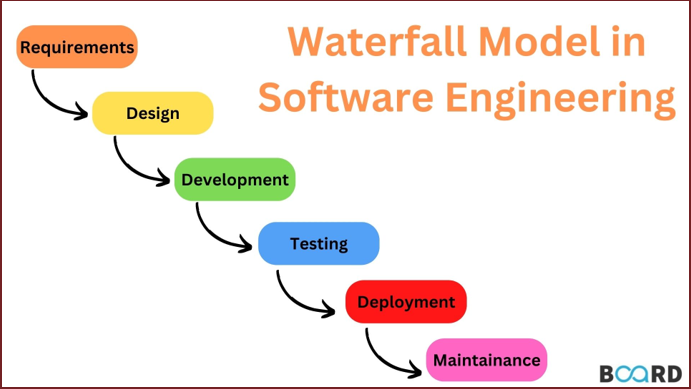
\includegraphics[width=0.6\textwidth]{Images/vandfald.png}
\end{center}


\subsection{Iterativ softwareudvikling}

Iterativ softwareudvikling er en metode hvor man gentager cyklusser af planlægning, implementering, test og evaluering.
Modsat vandfalsmodellen er det muligt at lave ændringer undervejs. Dette gør det muligt at lave store projekter
som kan være svære at overskue til start.

Iterativ softwareudvikling handler om at omfavne forandring i form af
tilbagemeldinger og tilpasning. Det kan godt være at kunden får nye ønsker
til produktet under testing og derfor skal man være klar til at lave
noget af det om.

\textbf{Fordele ved iterativ udvikling}

Det hjælper med tidlig lindring af risici (tekniske, krav, anvendelighed etc.)
Tidlige synlige fremskridt. Tidligt feedback, brugerinvolvering og engagement.
Udviklingsprocessen kan forbedres on the fly.


\begin{center}
	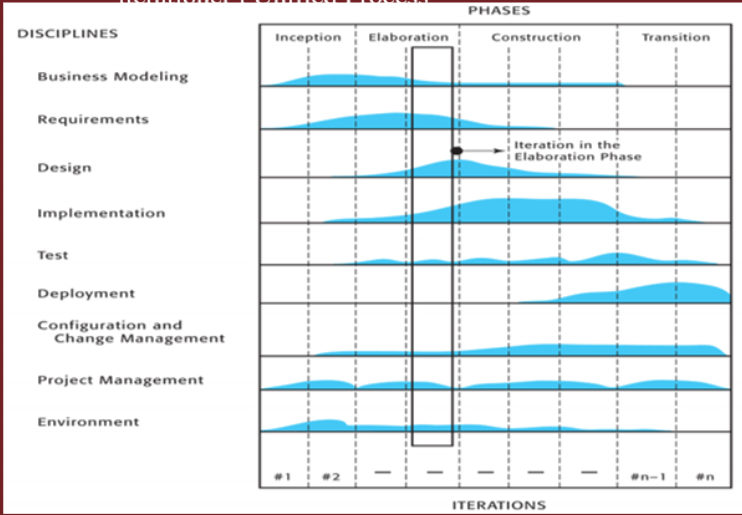
\includegraphics[width=0.8\textwidth]{Images/iterativ.png}
\end{center}


Iterativ softwareudvikling består af \textbf{4 faser}:

\begin{enumerate}
	\item{Inception - approximate vision, business case, scope, vague estimates}
	\item{Elaboration - Refined vision, iterative implementation of the core architecture,
	            resolution of high risks, identification of most requirements and scope, more realistic estimates.}
	\item{Construction - Iterative implementation of the remaining lower risk and easier elements
	            and preparation for deployment.}
	\item{Transition - Beta tests, deployment}
\end{enumerate}


Inception kan ses som begyndelse, der ikke behøver at tage lang tid.
Det er et indledende, hurtigt forløb, som besvarer følgende spørgsmål:

\begin{itemize}
	\item{Hvad er visionen og business casen for projektet?}
	\item{Kan det lade sig gøre?}
	\item{Køb og/eller byg?}
	\item{Første estimat. 100kr? eller millioner?}
	\item{Skal vi fortsætte eller stoppe}
\end{itemize}

\textbf{Keywords til inception}

\begin{itemize}

	\item{\textbf{Vision and business case}: Describes the high-level goals and constraints,
	            the business case, and provides an executive summary.}

	\item{\textbf{Use-case Model}: Describes the functional requirements, and related non-functional requirements.}

	\item{\textbf{Supplementary Specification}: Describes other requirements.}

	\item{\textbf{Risk list and Risk Management}: Describes the business,
	            techhnical resource, schedule risks, and ideas for their mitigation or response.}

	\item{\textbf{Prototypes and proof-of-concepts}: To clarify the vision, and validate technical ideas.}

	\item{\textbf{Iteration plan}: Describes what to do in the first elaboration iteration.}

	\item{\textbf{Phase Plan and software Dev. plan}: Low-precision guess for
	            elaboration phase duration and effort. Tools, people, education, and other resources.}

	\item{\textbf{Development case}: A description of the customized UP steps and artifacts
	            for this project. In the UP, one always customizes it for the project.}

\end{itemize}




\textbf{Discipliner}

\begin{enumerate}
	\item{Modellering af forretning}
	\item{Fastlæggelse af krav}
	\item{Design}
	\item{Implementering - skriv programmerne}
	\item{Test softwaren}
	\item{Deployment - integrer softwaren i virksomhedens organisation}
	\item{Konfigurations- og ændringsstyring}
	\item{Projektledelse}
	\item{Metode- og værktøjsunderstøttelse}
\end{enumerate}


\textbf{Resursefordeling}

\begin{center}
	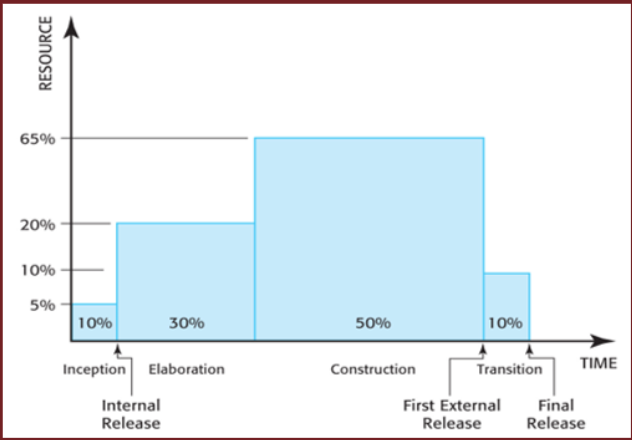
\includegraphics[width=0.8\textwidth]{Images/resursefordeling.png}
\end{center}

\textbf{Best practices til softwareudvikling}

Arbejd først på de mest risikable og værdiskabende features.
Involver brugerne kontinuerligt til evaluering, feedback og krav.
Byg en sammenhængende basisarkitektur i de tidlige iterationer.
Test ofte koden for at finde fejl. Modelér software visuelt (med UML).


\textbf{Krav FURPS+}

\begin{itemize}
	\item{Functional - features, capabilities, security}
	\item{Usability - human factors, help, documentation}
	\item{Reliability - frequency of failure, recoverability, predictability}
	\item{Performance - response times, throughput, accuracy, availability, resource usage}
	\item{Supportability - adaptability, maintainbility, internationalization, configurability}
\end{itemize}

The "+" in FURPS+ indicates supplementary and sub-factors, such as:
Implementation, interface, operations, packaging, legal.

